\documentclass[12pt,a4paper]{article}
\usepackage[left=4cm,right=3cm,top=3cm,bottom=3cm]{geometry}
\usepackage{mathptmx} % Times New Roman
\usepackage[T1]{fontenc}
\usepackage{textcomp}
\usepackage{amsmath}
\usepackage{amssymb}
\usepackage{graphicx}
\usepackage{float}
\usepackage{hyperref}
\usepackage{caption}
\captionsetup{justification=centering}
\renewcommand{\figurename}{Gambar}
\usepackage[none]{hyphenat}
\usepackage{tikz}
\usepackage{booktabs}
\usepackage{multirow}
\usepackage{enumitem}
\usepackage{varwidth} % Untuk better text wrapping
\usepackage{changepage} % Untuk adjusting margins on specific pages
\usepackage{algorithm}
\usepackage{algorithmic}
\usetikzlibrary{shapes.geometric, arrows, positioning, fit, calc, matrix}

% Pengaturan hyphenation - NO HYPHENATION AT ALL
\hyphenpenalty=10000
\exhyphenpenalty=10000
\tolerance=3000 % Increase tolerance
\emergencystretch=10em % Increase emergency stretch
\hyphenchar\font=-1
\sloppy
\hbadness=10000 % Suppress bad hbox warnings
\vbadness=10000 % Suppress bad vbox warnings

% Menghilangkan indentasi paragraf pertama setelah section
\setlength{\parindent}{0pt}
\setlength{\parskip}{6pt}


% Pengaturan jarak untuk subsection
\usepackage{titlesec}
\titleformat{\subsection}{\normalsize\bfseries}{\thesubsection}{1em}{}
\titlespacing*{\subsection}{0pt}{0pt}{0pt} % Tidak ada jarak sebelum atau setelah judul
\titlespacing*{\subsubsection}{1pt}{1pt}{0pt} % Tidak ada jarak sebelum atau setelah judul



% Definisi Style TikZ Terpusat
\tikzset{
    block/.style = {rectangle, draw, fill=blue!20, text width=8em, text centered, rounded corners, minimum height=3em},
    io/.style = {ellipse, draw, fill=yellow!20, text width=7em, text centered, minimum height=2em},
    process/.style = {rectangle, draw, fill=green!20, text width=14em, text centered, minimum height=2.5em},
    line/.style = {draw, -latex'},
    skipline/.style = {draw, ->, dashed}
}

\begin{document}

% ============================================================
% BAB IV: ANALISIS DAN DESAIN
% ============================================================

\vspace{2cm}
\begin{center}
{\fontsize{14}{16.8}\selectfont\textbf{BAB IV. Analisis dan Desain}}\\[1em]
\end{center}
\label{sec:analisis}
\addcontentsline{toc}{section}{BAB I PENDAHULUAN}
% penomoran sub bab
\setcounter{section}{4}
\setcounter{subsection}{0}
\vspace{2em}
% \subsection{Latar Belakang}
\label{subsec:analisis-desain}
\vspace{0.8em}

% akhir

\renewcommand{\thesection}{\Roman{section}}
\renewcommand{\thesubsection}{\thesection.\arabic{subsection}}
\renewcommand{\thesubsubsection}{\thesubsection.\arabic{subsubsection}}
% \setcounter{section}{3}
% \section{ANALISIS DAN DESAIN}
% \label{sec:analisis-desain}

Bab ini menguraikan rancangan solusi teknis yang diusulkan untuk restorasi dokumen terdegradasi dengan pendekatan Generative Adversarial Network yang dimodifikasi secara khusus untuk meningkatkan keterbacaan teks oleh model pengenalan tulisan tangan. Pembahasan dimulai dari analisis kebutuhan sistem (fungsional dan non-fungsional), dilanjutkan dengan rancangan arsitektur solusi yang mencakup desain Generator (U-Net), Recognizer (Transformer-based yang frozen), Diskriminator Dual-Modal (CNN+LSTM), dan fungsi loss multi-komponen (Adversarial + L1 + CTC). Selanjutnya, detail implementasi solusi diuraikan meliputi lingkungan eksperimen, persiapan dataset (ground truth untuk pengenalan tulisan tangan dan sintetis untuk GAN), implementasi arsitektur model dalam TensorFlow/Keras, prosedur training dengan optimasi alternating, dan justifikasi pemilihan hyperparameter melalui studi ablasi.

\subsection{Analisis Kebutuhan Sistem} % This will be numbered as 4.1

Berdasarkan rumusan masalah dan tujuan penelitian, sistem restorasi dokumen yang akan dibangun harus memenuhi serangkaian kebutuhan fungsional dan non-fungsional. Kebutuhan ini menjadi acuan dalam perancangan arsitektur dan tolok ukur dalam evaluasi akhir, sejalan dengan tahapan DSRM.

\subsubsection{Kebutuhan Fungsional} % This will be numbered as 4.1.1 Kebutuhan fungsional mendefinisikan fungsi atau kemampuan spesifik yang harus dimiliki oleh sistem.

Kebutuhan fungsional mendefinisikan fungsi spesifik yang harus dimiliki oleh sistem GAN-HTR untuk restorasi dokumen terdegradasi secara efektif. Delapan kebutuhan fungsional yang diidentifikasi mencakup tiga kategori:

\begin{enumerate}
    \item Kemampuan inti pembelajaran mesin untuk restorasi visual dan pengenalan teks,
    \item Kemampuan pemrosesan untuk menangani batch inference dan dataset sintetis,
    \item Kemampuan integrasi sistem untuk input/output terstandar dan antarmuka fleksibel.
\end{enumerate}
Setiap kebutuhan dirancang untuk memastikan sistem tidak hanya secara teknis mampu melakukan restorasi, tetapi juga praktis untuk digunakan dalam lingkungan produksi dan dapat diintegrasikan dengan sistem lain.

\begin{table}[htbp!]
\centering
\small
\caption{Ringkasan Kebutuhan Fungsional Sistem GAN-HTR}
\label{tab:functional_requirements}
\begin{tabular}{p{0.07\textwidth}p{0.20\textwidth}p{0.68\textwidth}}
\toprule
\textbf{Kode} & \textbf{Nama Kebutuhan} & \textbf{Deskripsi dan Detail Spesifikasi} \\
\midrule
FR-1 & Kemampuan Restorasi Gambar & Menerima input gambar dokumen terdegradasi dan menghasilkan output gambar versi restorasi yang lebih bersih secara visual. \\
\midrule
FR-2 & Penanganan Berbagai Degradasi & Menangani 4 jenis degradasi utama: tembusan tinta, pemudaran, noda, dan efek buram. \\
\midrule
FR-3 & Integrasi dengan Proses HTR & Gambar restorasi dapat diproses oleh model HTR untuk menghasilkan transkripsi teks. \\
\midrule
FR-4 & Inferensi Batch \newline Processing & Memproses dokumen terdegradasi secara batch dengan output: (1) Gambar restorasi penuh, (2) File teks (.txt), (3) File metadata (.json). \\
\midrule
FR-5 & Dukungan Dataset Sintetis & Menyertakan pipeline pembuatan dataset sintetis terdegradasi dari gambar bersih. \\
\midrule
FR-6 & Output Terdefinisi & Format output konsisten: (1) Visual: PNG/TIFF 300 DPI, (2) Text: UTF-8 dengan confidence 0.0-1.0, (3) Quality: PSNR/SSIM, (4) Error messages. \\
\midrule
FR-7 & Input Data Fleksibel & Menangani: (1) Format: JPG, PNG, TIFF, PDF, (2) Validasi: resolusi min 128x1024px, (3) Recovery: skip corrupted files, (4) Preprocessing: grayscale dan noise reduction. \\[-0.5em]
   & & \textit{Catatan: Semua input divalidasi sebelum diproses.} \\
\midrule
FR-8 & Integrasi Sistem & Menyediakan: (1) CLI dengan parameter, (2) Python API, (3) Configuration YAML/JSON, (4) Structured logging. \\
\bottomrule
\end{tabular}
\end{table}

\vspace{1.5em}

\clearpage
\subsubsection{Kebutuhan Non-Fungsional} % This will be numbered as 4.1.2 Kebutuhan non-fungsional mendefinisikan kriteria kualitas atau batasan performa dari sistem.

Kebutuhan non-fungsional mendefinisikan kriteria kualitas dan batasan performa sistem GAN-HTR. Empat kebutuhan non-fungsional yang ditetapkan mengukur aspek kualitatif dan kuantitatif performa sistem:

\begin{enumerate}
    \item Kualitas Visual mengukur kesamaan dengan ground truth menggunakan PSNR dan SSIM,
    \item Keterbacaan Teks sebagai metrik utama keberhasilan sistem melalui penurunan CER,
    \item Efisiensi Waktu untuk memastikan kepraktisan penggunaan,
    \item Reproduktifitas untuk menjamin konsistensi dan keandalan hasil eksperimen.
\end{enumerate}
Target performa ditetapkan berdasarkan studi literatur dan kebutuhan praktis implementasi.

\begin{table}[htbp!]
\centering
\small
\caption{Ringkasan Kebutuhan Non-Fungsional Sistem GAN-HTR}
\label{tab:non_functional_requirements}
\begin{tabular}{p{0.07\textwidth}p{0.25\textwidth}p{0.65\textwidth}}
\toprule
\textbf{Kode} & \textbf{Nama Requirement} & \textbf{Deskripsi dan Target Performa} \\
\midrule
NFR-1 & Kualitas Visual Restorasi & Kualitas visual gambar hasil restorasi vs ground truth harus mencapai: (1) PSNR rata-rata $\geq$ 35 dB, (2) SSIM rata-rata $\geq$ 0.90 pada dataset validasi. \\[0.3em]
   & & \textit{Target berdasarkan studi literatur dan uji coba awal.} \\
\midrule
NFR-2 & Peningkatan Keterbacaan Teks & Sistem harus meningkatkan akurasi transkripsi HTR secara signifikan: CER menunjukkan penurunan minimal 25\% dibandingkan CER pada gambar terdegradasi asli. \\[0.3em]
   & & \textit{Dihitung sebagai: (CER\_asli - CER\_restorasi)/CER\_asli $\times$ 100\%}. \\
\midrule
NFR-3 & Performa Waktu Inferensi & Waktu inferensi untuk satu gambar dokumen tunggal pada NVIDIA RTX A4000 tidak boleh melebihi 15 detik untuk memastikan kepraktisan penggunaan. \\
\midrule
NFR-4 & Reproduktifitas & Proses training dan evaluasi harus dapat direproduksi dengan lingkungan perangkat lunak dan dependensi yang didefinisikan secara jelas (melalui file \texttt{pyproject.toml}). \\
\bottomrule
\end{tabular}
\end{table}

\vspace{1.5em}

Berdasarkan Tabel \ref{tab:functional_requirements} dan Tabel \ref{tab:non_functional_requirements}, sistem GAN-HTR yang akan dikembangkan harus memenuhi total 12 kebutuhan (8 fungsional dan 4 non-fungsional) yang mencakup aspek visual, tekstual, performa, dan integrasi sistem.

\subsection{Rancangan Arsitektur} % This will be numbered as 4.2

Rancangan solusi bertujuan untuk membangun sebuah model generatif yang tidak hanya mampu membersihkan gambar dari kerusakan visual, tetapi juga secara eksplisit dioptimalkan untuk menghasilkan gambar yang keterbacaan teksnya maksimal. Untuk mencapai tujuan ini, arsitektur GAN standar dimodifikasi dengan memperkenalkan dua elemen kunci: (1) Diskriminator dual-modal yang menilai koherensi antara gambar dan teks, dan (2) Fungsi loss gabungan yang mencakup loss dari model pengenalan tulisan tangan.

\subsubsection{Gambaran Umum Arsitektur} % This will be numbered as 4.2.1 
Arsitektur yang diusulkan terdiri dari tiga komponen utama yang berinteraksi dalam sebuah kerangka adversarial, seperti yang diilustrasikan pada Gambar \ref{fig:arch_overview}. Ketiga komponen tersebut adalah:
\begin{enumerate}[nosep]
    \item Generator (G): Sebuah model dengan arsitektur U-Net yang bertugas menerima gambar dokumen terdegradasi dan menghasilkan versi restorasi dari gambar tersebut.
    \item Recognizer (R): Sebuah model HTR berbasis Transformer yang sudah terlatih dan dibekukan (frozen). Tujuannya bukan untuk dilatih, melainkan untuk "membaca" teks dari gambar hasil restorasi dan memberikan sinyal loss terkait keterbacaan.
    \item Diskriminator (D): Sebuah model Diskriminator dual-modal yang menjadi inti dari penelitian ini. Tidak seperti diskriminator pada umumnya yang hanya menerima input gambar, diskriminator ini menerima pasangan \textit{(gambar, representasi teks)} untuk menilai apakah sebuah gambar "asli" dan apakah teks di dalamnya koheren.
\end{enumerate}

\begin{figure}[htbp!]
\centering
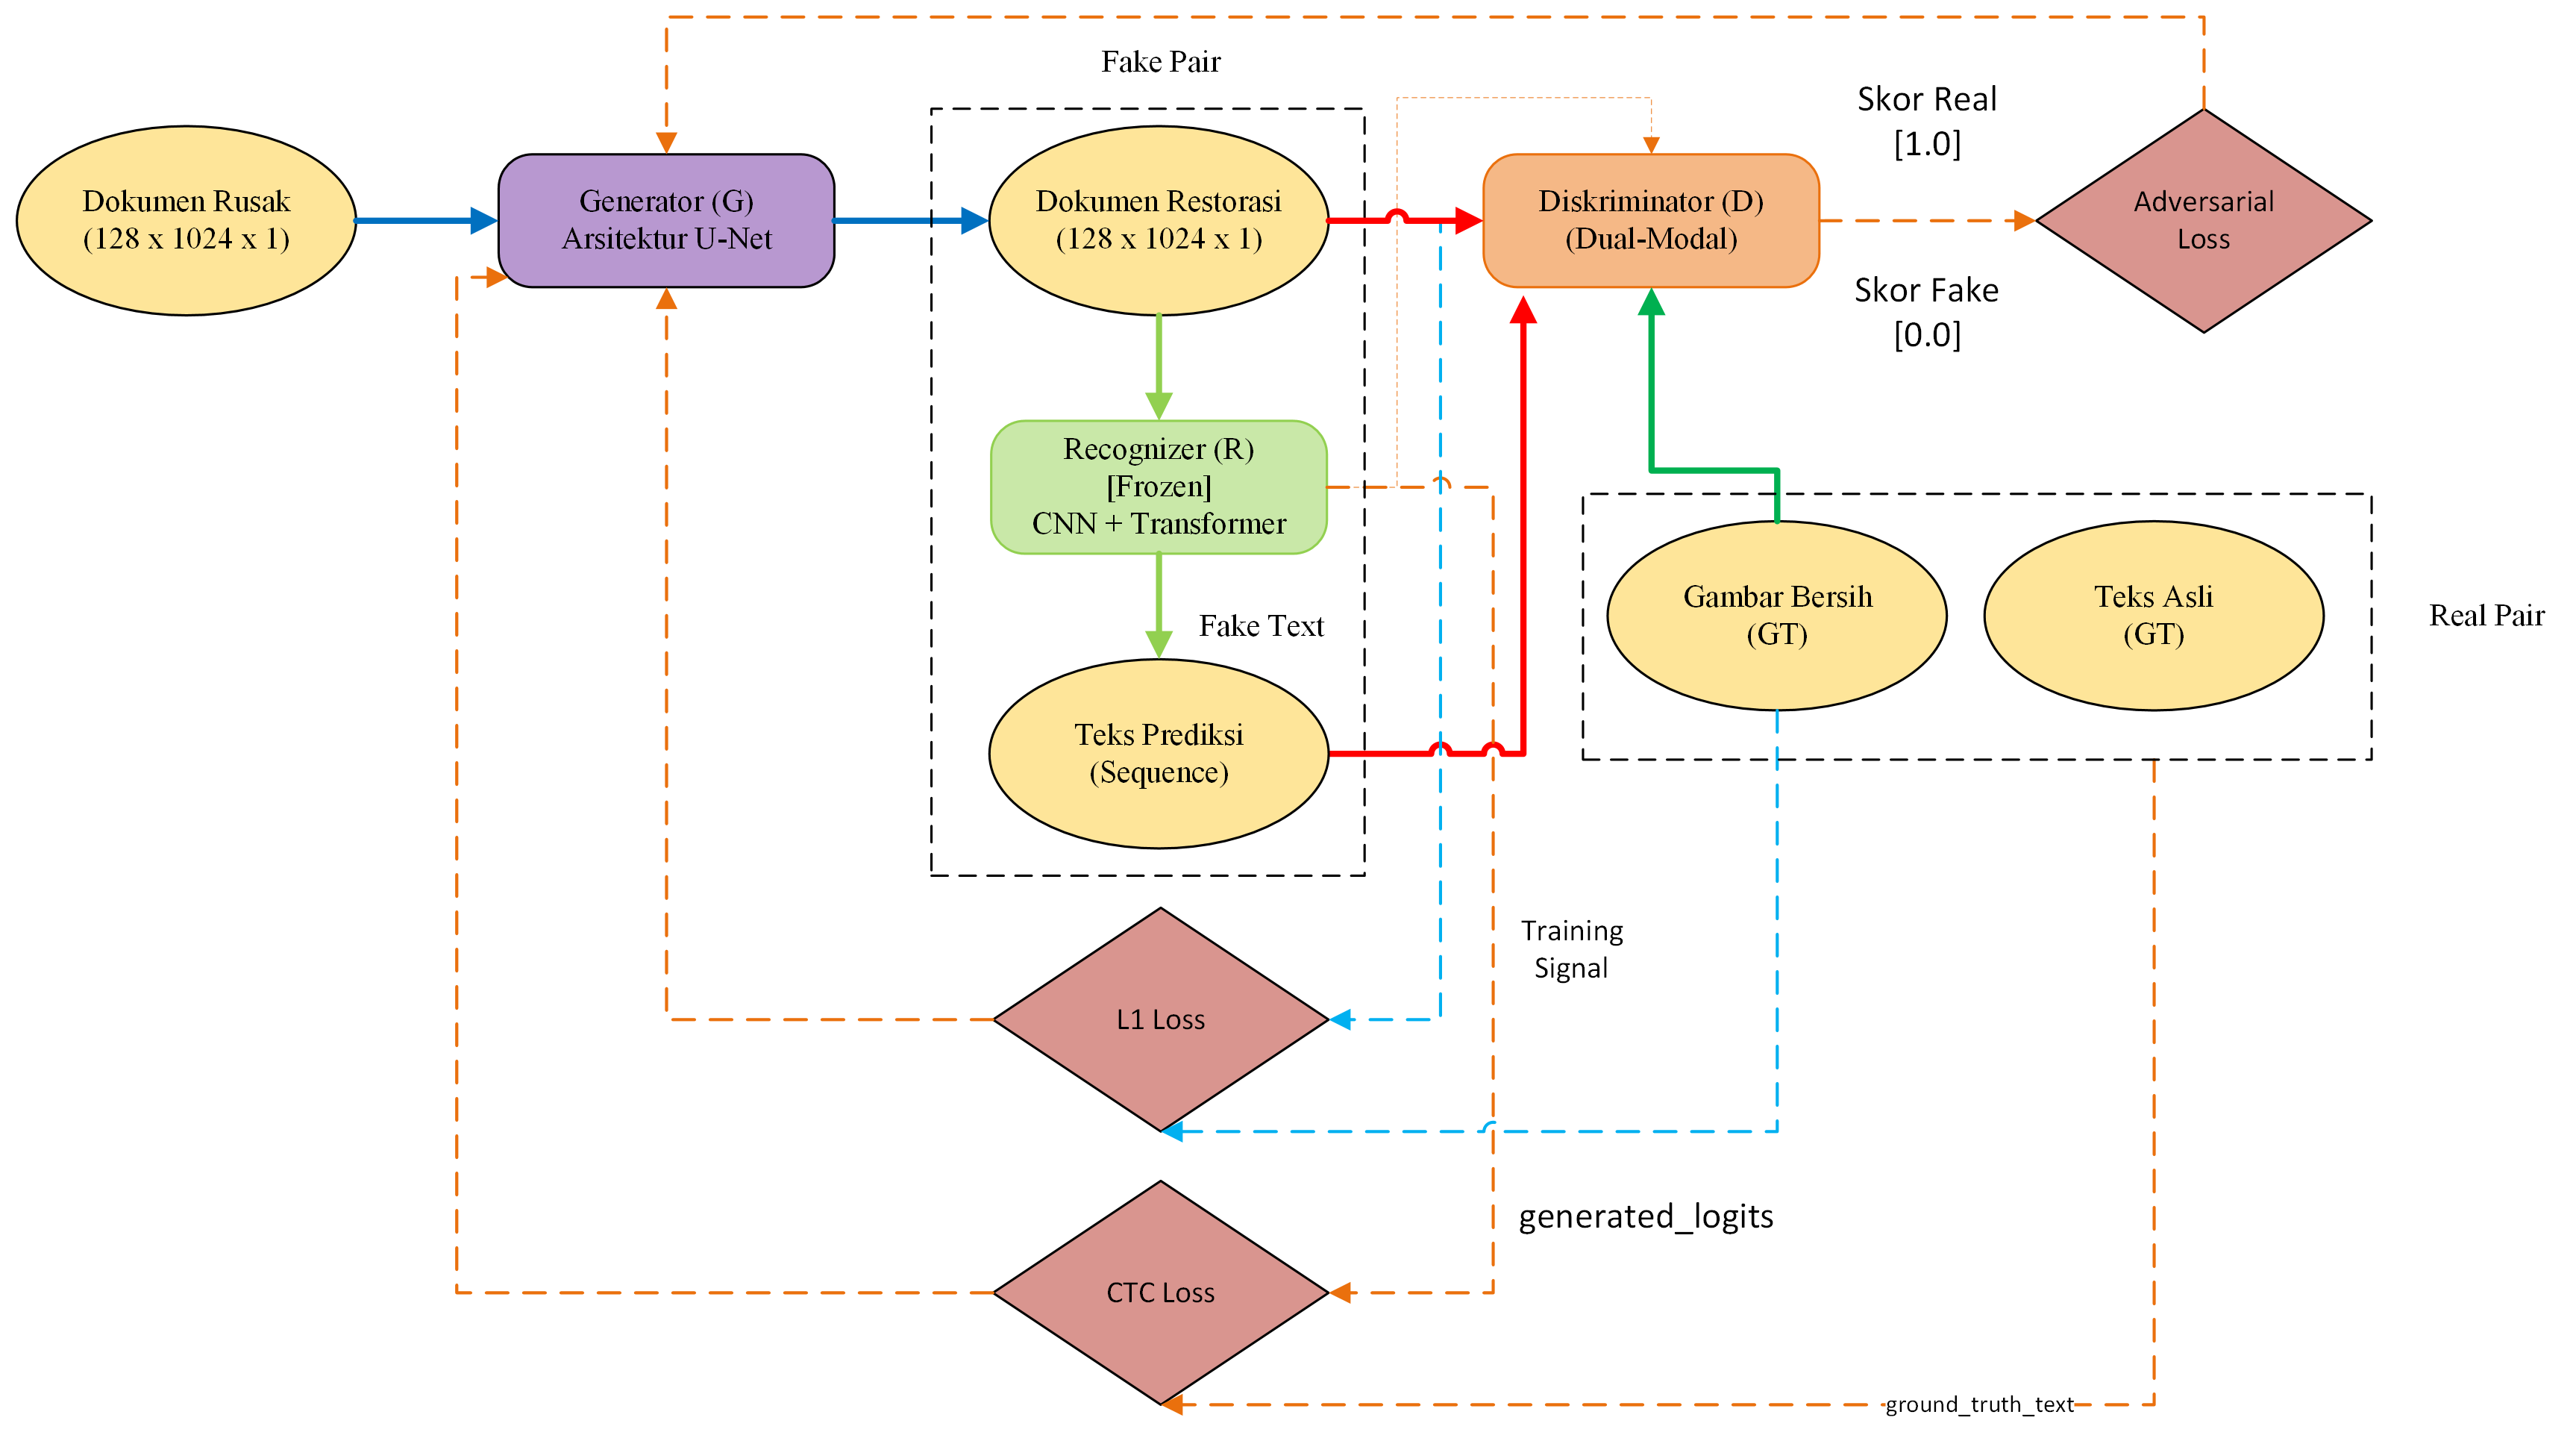
\includegraphics[width=0.9\textwidth]{images/ArsitekturUmum.png}
\caption{Diagram alur arsitektur GAN. Diagram menunjukkan input untuk setiap komponen loss: L1 Loss membandingkan dua gambar, CTC Loss membandingkan dua sekuens teks, dan Adversarial Loss berasal dari Diskriminator.}
\label{fig:arch_overview}
\end{figure}

\subsubsection{Desain Generator} % This will be numbered as 4.2.2 Untuk komponen Generator (G), arsitektur yang dipilih adalah U-Net. Arsitektur ini merupakan standar de-facto untuk berbagai tugas translasi gambar-ke-gambar (image-to-image translation), termasuk restorasi, karena efektivitasnya dalam merekonstruksi detail halus pada gambar output. Struktur U-Net terdiri dari dua jalur utama: jalur kontraksi (encoder) dan jalur ekspansi (decoder), yang dihubungkan oleh \textit{skip connections}, seperti diilustrasikan pada Gambar \ref{fig:unet_arch}.

\begin{itemize}
    \item Jalur Encoder: Berfungsi seperti jaringan konvolusi pada umumnya untuk mengekstraksi fitur dari gambar input. Melalui serangkaian blok konvolusi dan operasi \textit{max-pooling}, resolusi spasial gambar secara bertahap dikurangi (downsampling) sementara kedalaman fitur (jumlah channel) ditingkatkan. Proses ini memungkinkan model untuk menangkap informasi kontekstual dari gambar

    \item Jalur Decoder: Bertugas untuk merekonstruksi gambar output dari representasi fitur yang telah dipelajari oleh encoder. Melalui serangkaian blok \textit{upsampling} dan konvolusi, resolusi spasial gambar secara bertahap ditingkatkan hingga kembali ke ukuran aslinya.

    \item Skip Connections: Ini adalah fitur utama dari arsitektur U-Net. Koneksi ini menghubungkan secara langsung feature map dari lapisan di jalur encoder ke lapisan yang bersesuaian di jalur decoder. Dengan meneruskan informasi dari lapisan awal (yang kaya akan detail spasial) ke lapisan akhir, U-Net mampu mengatasi hilangnya informasi detail yang sering terjadi pada arsitektur encoder-decoder standar. Untuk tugas restorasi dokumen, ini sangat penting untuk menjaga ketajaman dan keutuhan gurat-gurat tipis pada karakter tulisan tangan.
\end{itemize}
\begin{figure}[H] % Memaksa gambar muncul di sini setelah penjelasan generator
\centering
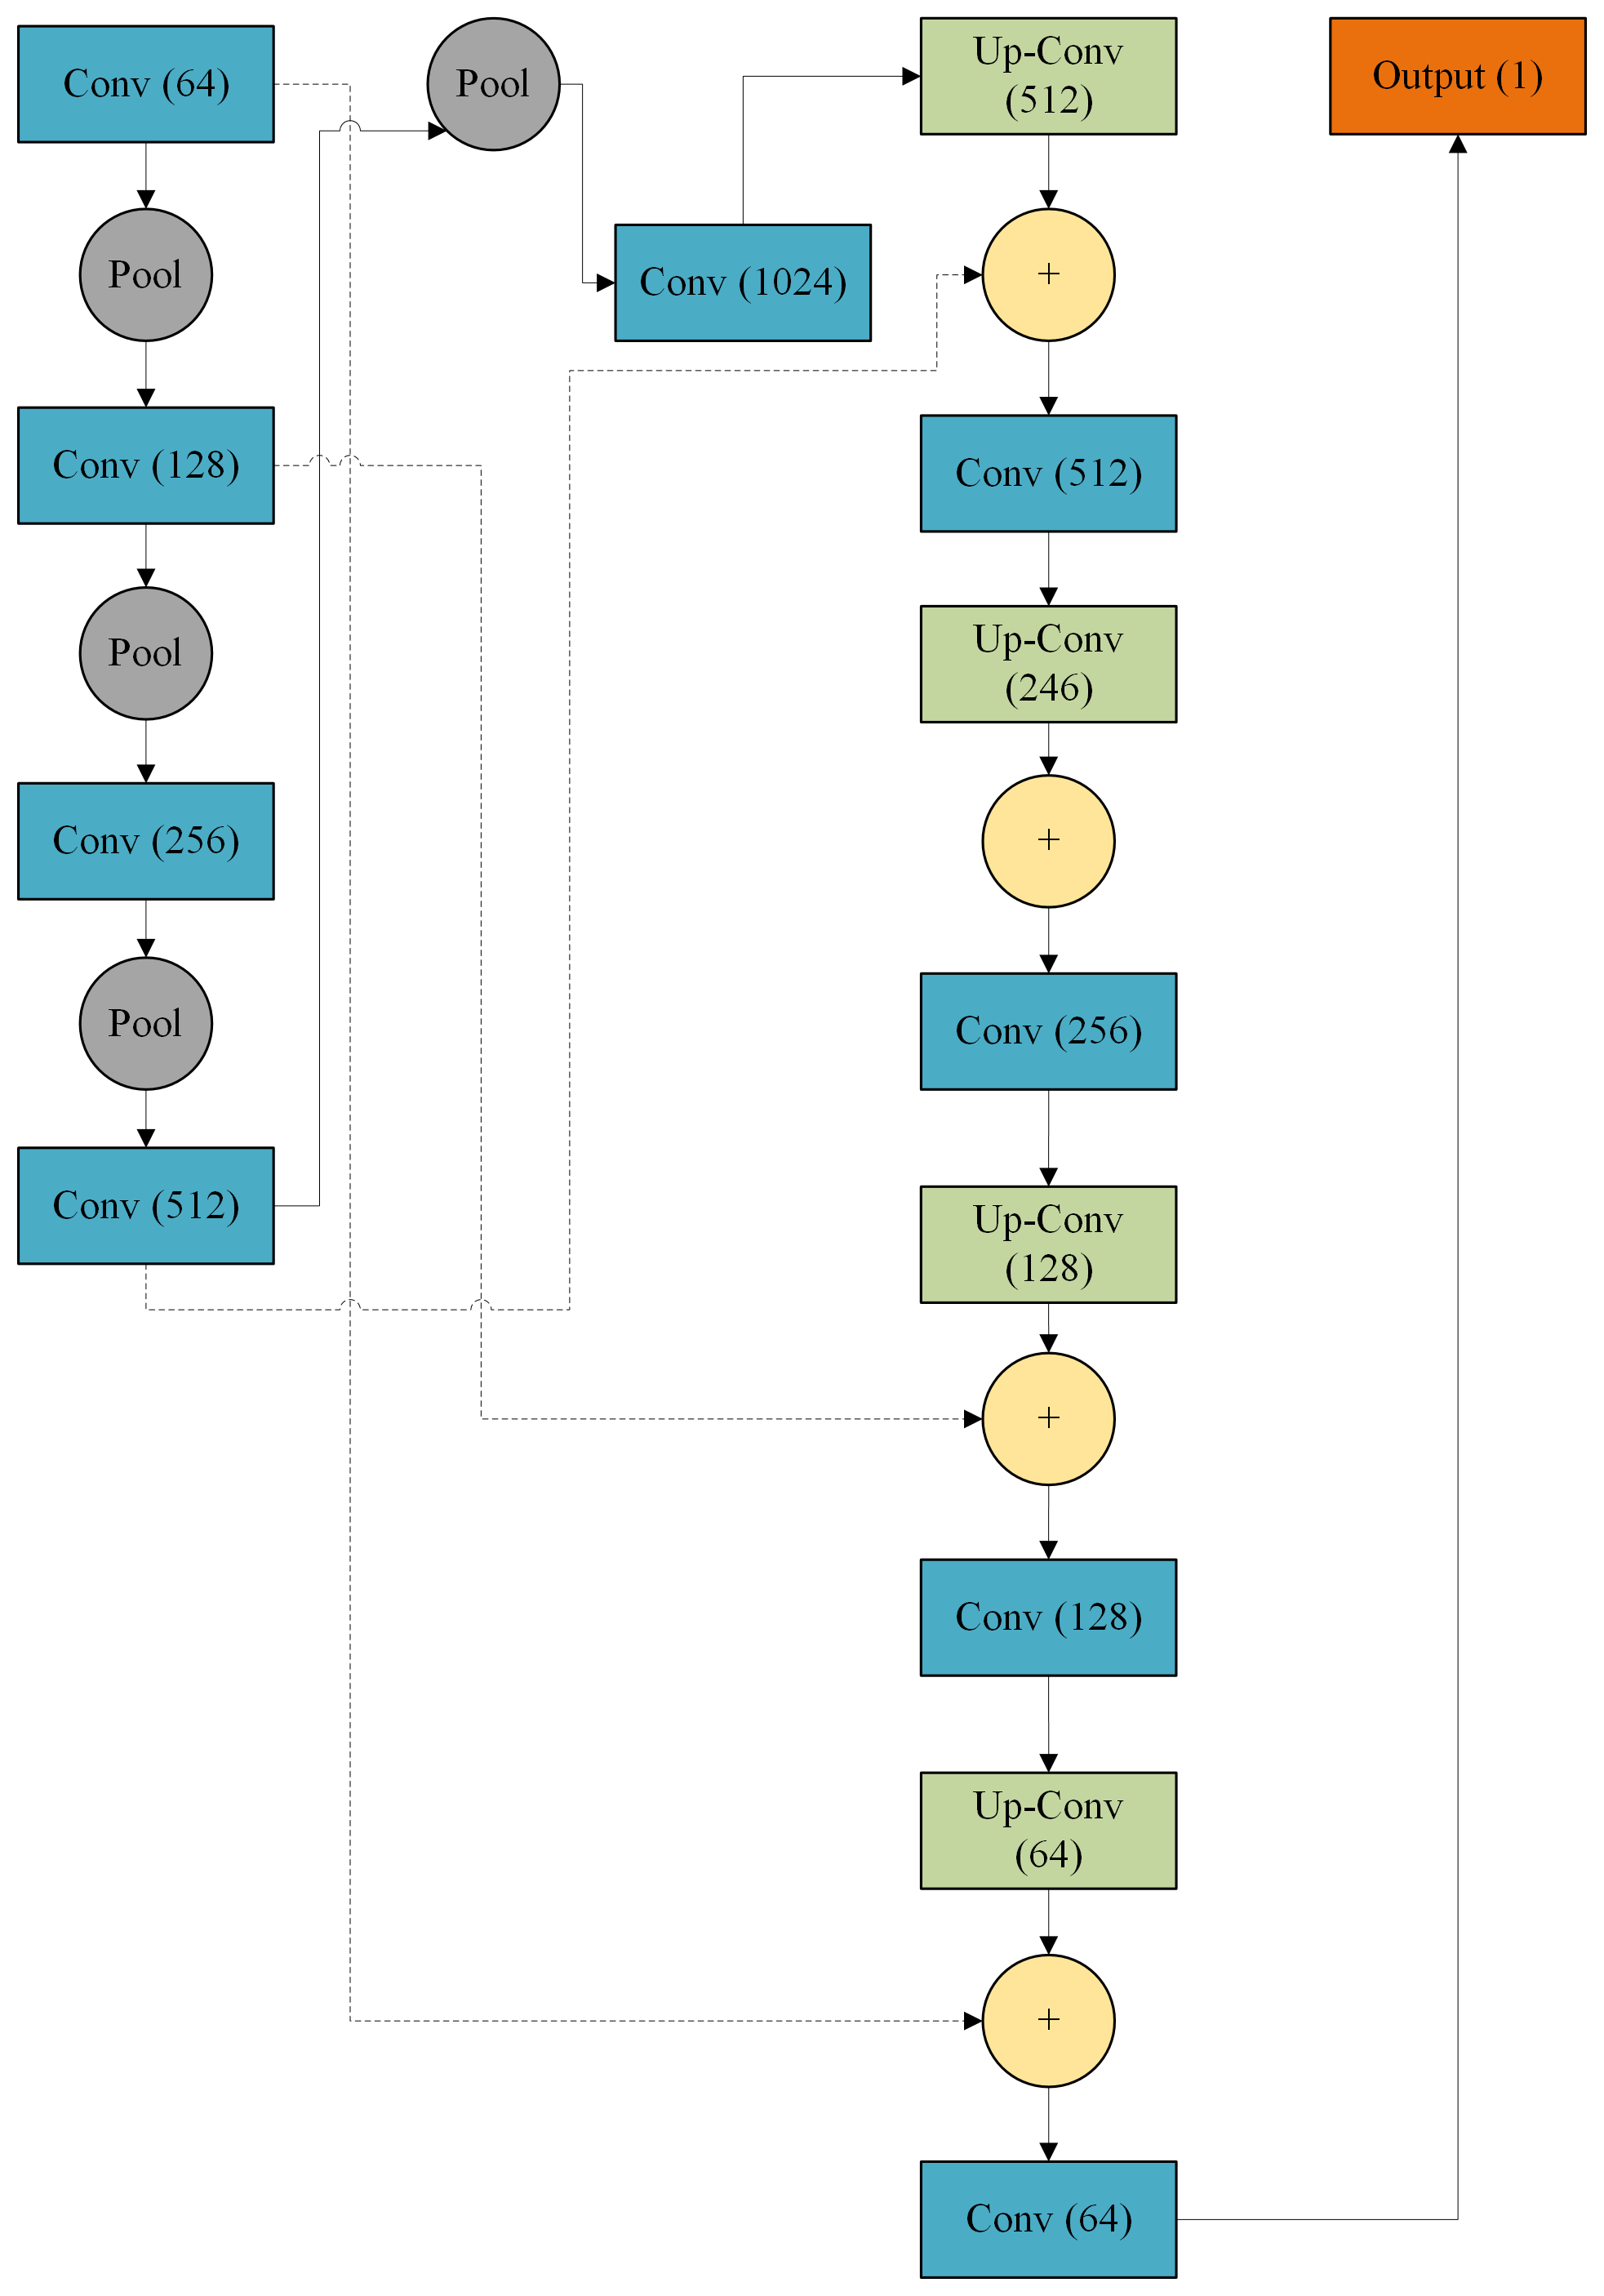
\includegraphics[width=0.9\textwidth, height=0.45\textheight, keepaspectratio]{images/generator.png}
\caption{Diagram arsitektur U-Net yang digunakan sebagai Generator.}
\label{fig:unet_arch}
\end{figure}

\subsubsection{Desain Recognizer} % This will be numbered as 4.2.3
Komponen Recognizer (R) memainkan peran khusus dan esensial dalam arsitektur yang diusulkan. Berbeda dengan komponen lain, Recognizer tidak dilatih selama proses training GAN. Sebaliknya, komponen ini merupakan sebuah model Handwritten Text Recognition (HTR) berbasis Transformer yang telah dilatih sebelumnya (\textit{pre-trained}) dan bobotnya dibekukan (\textit{frozen}) atau diatur sebagai \textit{non-trainable}.

\paragraph{Fungsi Utama dan Peran dalam Arsitektur}

Recognizer berfungsi sebagai evaluator keterbacaan teks yang objektif. Komponen ini menerima gambar hasil restorasi dari Generator dan menghasilkan distribusi probabilitas karakter untuk mengukur keterbacaan hasil restorasi. Output dari Recognizer digunakan untuk dua tujuan:

\begin{enumerate}[nosep]
    \item Sebagai input teks untuk Diskriminator, yang menilai koherensi antara gambar dan teks yang dikenali.
    \item Sebagai input untuk kalkulasi CTC Loss, yang secara langsung mengukur seberapa dapat dibaca gambar hasil restorasi.
\end{enumerate}

% \paragraph{Justifikasi Frozen Recognizer Philosophy}

Keputusan untuk membekukan bobot Recognizer (frozen) selama training GAN didasarkan pada tiga pertimbangan ilmiah yang krusial:

\begin{enumerate}[nosep]
    \item \textbf{Objective Evaluator:} Recognizer dengan bobot frozen berfungsi sebagai evaluator objektif dengan metrik yang stabil dan konsisten. Jika bobot recognizer dilatih ulang, metrik keterbacaan akan berubah-ubah seiring training, sehingga kehilangan fungsinya sebagai ground truth evaluasi.
    
    \item \textbf{Catastrophic Forgetting Prevention:} Melatih recognizer secara simultan dengan GAN dapat menyebabkan catastrophic forgetting, di mana recognizer kehilangan kemampuan mengenali karakter yang telah dipelajari sebelumnya karena terfokus pada gambar restorasi yang terus berubah.
    
    \item \textbf{Focused Visual Optimization:} Dengan membekukan recognizer, optimasi Generator terfokus pada adaptasi visual untuk meningkatkan keterbacaan, bukan melatih recognizer untuk membaca lebih baik. Ini memastikan bahwa peningkatan berasal dari kualitas gambar, bukan dari adaptasi recognizer.
\end{enumerate}

\begin{figure}[H]
\centering
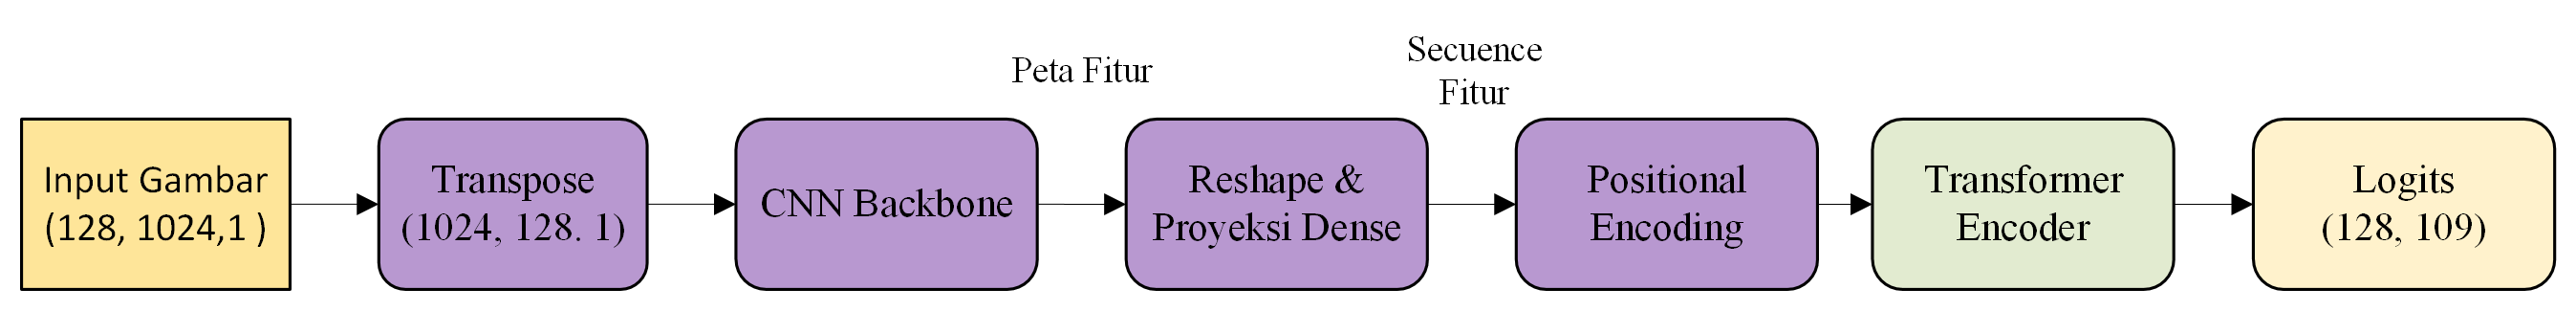
\includegraphics[width=\textwidth, height=1\textheight, keepaspectratio]{images/Recognizer.png}
\caption{Diagram arsitektur Recognizer berbasis CNN+Transformer untuk ekstraksi fitur dan pengenalan teks.}
\label{fig:recognizer_arch}
\end{figure}

\paragraph{Arsitektur High-Level}

Recognizer menggunakan arsitektur CNN+Transformer yang dirancang khusus untuk dokumen kuno:

\begin{itemize}
    \item CNN Backbone: Mengekstrak fitur visual hierarkis dari stroke dasar hingga kompleksitas karakter
    \item Transformer Encoder: Menangkap dependensi jarak jauh dan konteks linguistik dengan multi-head attention
    \item CTC Output Layer: Menghasilkan probabilitas karakter untuk setiap timestep
\end{itemize}

Detail justifikasi pemilihan arsitektur CNN+Transformer untuk kasus paleografi telah dibahas secara komprehensif pada Bab 2.3.4.
\subsubsection{Detail Arsitektur Recognizer}
\label{subsubsec:detail-arsitektur-recognizer}

Recognizer mengimplementasikan arsitektur Hybrid CNN-Transformer yang dirancang untuk ekstraksi fitur visual hierarkis dan pemodelan dependensi sekuensial pada dokumen paleografi. Arsitektur ini terdiri dari tiga komponen utama: CNN backbone untuk ekstraksi fitur, Transformer encoder untuk context modeling, dan CTC output layer untuk decoding.

\paragraph{CNN Backbone: 8-Layer Feature Extraction}

CNN backbone mengekstrak representasi visual hierarkis melalui 8 convolutional layers yang tersusun dalam 4 stages dengan progressive pooling strategy:

\begin{table}[H]
\centering
\caption{Spesifikasi layer-by-layer CNN Backbone (8 convolutional layers)}
\label{tab:recognizer-cnn-detailed}
\scriptsize
\begin{tabular}{|l|l|l|l|l|l|}
\hline
\textbf{Stage} & \textbf{Layer} & \textbf{Kernel} & \textbf{Filters} & \textbf{Activation} & \textbf{Output Shape} \\
\hline
\multirow{3}{*}{Stage 1} & Conv2D-1 & 3×3, stride=1 & 64 & GELU & (128, 1024, 64) \\
\cline{2-6}
 & Conv2D-2 & 3×3, stride=1 & 64 & GELU & (128, 1024, 64) \\
\cline{2-6}
 & MaxPool2D-1 & 2×2 & - & - & (64, 512, 64) \\
\hline
\multirow{3}{*}{Stage 2} & Conv2D-3 & 3×3, stride=1 & 128 & GELU & (64, 512, 128) \\
\cline{2-6}
 & Conv2D-4 & 3×3, stride=1 & 128 & GELU & (64, 512, 128) \\
\cline{2-6}
 & MaxPool2D-2 & 2×2 & - & - & (32, 256, 128) \\
\hline
\multirow{3}{*}{Stage 3} & Conv2D-5 & 3×3, stride=1 & 256 & GELU & (32, 256, 256) \\
\cline{2-6}
 & Conv2D-6 & 3×3, stride=1 & 256 & GELU & (32, 256, 256) \\
\cline{2-6}
 & MaxPool2D-3 & (2,1) & - & - & (16, 256, 256) \\
\hline
\multirow{3}{*}{Stage 4} & Conv2D-7 & 3×3, stride=1 & 512 & GELU & (16, 256, 512) \\
\cline{2-6}
 & Conv2D-8 & 3×3, stride=1 & 512 & GELU & (16, 256, 512) \\
\cline{2-6}
 & MaxPool2D-4 & (2,1) & - & - & (8, 256, 512) \\
\hline
\multicolumn{6}{|l|}{\textbf{Sequence Projection}} \\
\hline
\multicolumn{2}{|l|}{GlobalAvgPool (height)} & \multicolumn{4}{l|}{Collapse height dimension → (256, 512)} \\
\hline
\multicolumn{2}{|l|}{Dense Projection} & \multicolumn{4}{l|}{512 → 512 dengan LayerNorm} \\
\hline
\end{tabular}
\end{table}

\textbf{Design Rationale CNN:}
\begin{itemize}[nosep]
    \item \textbf{8 Layers vs Standard 5-6:} Dokumen paleografi memiliki kompleksitas stroke yang tinggi, memerlukan ekstraksi fitur lebih dalam untuk menangkap variasi gaya tulisan abad 16-18.
    \item \textbf{Progressive Pooling (2,2)→(2,2)→(2,1)→(2,1):} Preservasi dimensi horizontal (width) lebih agresif untuk mempertahankan resolusi sekuensial yang penting dalam HTR.
    \item \textbf{GELU Activation:} Terbukti lebih efektif untuk vision transformer dibanding ReLU karena smooth gradient flow.
    \item \textbf{NO Residual Connections:} Arsitektur ini didesain untuk sequential feature extraction tanpa skip connections untuk menghindari kompleksitas berlebihan pada model baseline.
\end{itemize}

\paragraph{Transformer Encoder: 6-Layer Sequence Modeling}

Transformer encoder menangkap dependensi jarak jauh dan konteks linguistik melalui 6 stacked layers dengan multi-head self-attention:

\begin{table}[H]
\centering
\caption{Spesifikasi Transformer Encoder (6 layers)}
\label{tab:recognizer-transformer-detailed}
\small
\begin{tabular}{|l|l|l|}
\hline
\textbf{Component} & \textbf{Specification} & \textbf{Design Choice} \\
\hline
Number of Layers & 6 & Standard depth untuk HTR \\
\hline
Model Dimension ($d_{model}$) & 512 & Match CNN output dimension \\
\hline
Attention Heads & 8 & Head dimension = 64 (512/8) \\
\hline
FFN Dimension ($d_{ff}$) & 2048 & 4× expansion ratio (standard) \\
\hline
Positional Encoding & \textbf{Learned Embedding} & Trainable, adaptif ke variasi layout \\
\hline
Dropout (Attention) & 0.20 & Regularisasi pada attention weights \\
\hline
Dropout (FFN) & 0.20 & Regularisasi pada feed-forward \\
\hline
Layer Normalization & Pre-LN & Stabilitas training (before attention) \\
\hline
Activation (FFN) & GELU & Smooth non-linearity \\
\hline
\end{tabular}
\end{table}

\textbf{Design Rationale Transformer:}
\begin{itemize}[nosep]
    \item \textbf{Learned Positional Embedding vs Sinusoidal:} Learned embedding dapat beradaptasi dengan karakteristik spasial unik dokumen paleografi (spacing variabel, distorsi geometris).
    \item \textbf{6 Layers:} Balance antara kapasitas model dan overfitting risk pada dataset terbatas ($\sim$50K samples).
    \item \textbf{Pre-LN:} Layer normalization sebelum attention terbukti lebih stabil untuk deep transformer dibanding Post-LN.
\end{itemize}

\paragraph{CTC Output Layer dan Decoding}

\begin{table}[H]
\centering
\caption{CTC Output Layer specification}
\label{tab:recognizer-ctc-spec}
\small
\begin{tabular}{|l|p{10cm}|}
\hline
\textbf{Component} & \textbf{Specification} \\
\hline
Output Dense Layer & Dense(charset\_size + 1) dengan softmax activation \\
\hline
Charset Size & 95 karakter (A-Z, a-z, 0-9, punctuation, special chars) \\
\hline
Blank Token & Index 0 (CTC blank untuk non-emission) \\
\hline
Loss Function & CTC Loss dengan label smoothing $\epsilon$=0.1 \\
\hline
Decoding Strategy & Greedy decoding (argmax per timestep) untuk inference \\
\hline
Label Smoothing & $\epsilon$=0.1 → entropy regularization untuk robustness \\
\hline
\end{tabular}
\end{table}

\paragraph{Regularization dan Training Configuration}

\begin{table}[H]
\centering
\caption{Regularization dan Optimizer configuration Recognizer}
\label{tab:recognizer-training-config}
\small
\begin{tabular}{|l|l|}
\hline
\textbf{Parameter} & \textbf{Value} \\
\hline
Optimizer & AdamW (decoupled weight decay) \\
\hline
Learning Rate & 3×10$^{-4}$ (peak after warmup) \\
\hline
Weight Decay & 2×10$^{-4}$ (L2 regularization) \\
\hline
LR Schedule & WarmupCosineDecay (5 epochs warmup, min\_lr=1×10$^{-7}$) \\
\hline
Gradient Clipping & Norm clipping at 1.0 (prevent explosion) \\
\hline
Batch Size & 32 (optimal untuk GPU memory vs convergence) \\
\hline
Dropout (CNN) & 0.10-0.20 (progressive per stage) \\
\hline
Dropout (Transformer) & 0.20 (attention + FFN) \\
\hline
Label Smoothing & 0.1 (entropy regularization) \\
\hline
Early Stopping & Patience=15 epochs, monitor val\_loss \\
\hline
Data Augmentation & Brightness ±20\%, Contrast 0.8-1.2, Noise $\sigma$=0.08 \\
\hline
\end{tabular}
\end{table}

\paragraph{Performance Metrics dan Target}

\begin{table}[H]
\centering
\caption{Target performance metrics Recognizer}
\label{tab:recognizer-performance-target}
\small
\begin{tabular}{|l|l|l|}
\hline
\textbf{Metric} & \textbf{Target} & \textbf{Achieved (Baseline Stage 3)} \\
\hline
Character Error Rate (CER) & $<$ 15\% & $\sim$33\% \\
\hline
Word Error Rate (WER) & $<$ 25\% & $\sim$45\% \\
\hline
Inference Speed & $<$ 100ms/image & $\sim$85ms (RTX A4000) \\
\hline
Model Size & $<$ 50MB & 48.2 MB \\
\hline
\end{tabular}
\end{table}

\textbf{Catatan:} Spesifikasi lengkap parameter count per-layer, dimensional flow, dan implementation code tersedia pada Lampiran A (Tabel \ref{tab:appendix-cnn-detailed}, \ref{tab:appendix-transformer-detailed}).

\subsubsection{Desain Diskriminator Dual-Modal} % This will be numbered as 4.2.4

Inovasi utama dalam rancangan solusi ini terletak pada arsitektur Diskriminator (D). Berbeda dengan diskriminator pada GAN konvensional yang hanya menilai realisme sebuah gambar (unimodal), diskriminator yang diusulkan bersifat dual-modal. Tujuannya tidak hanya untuk membedakan gambar asli dari gambar palsu, tetapi juga untuk menilai koherensi antara konten visual sebuah gambar dengan konten semantik dari teks yang diekstraksi dari gambar tersebut.

Diskriminator ini menerima sepasang input: sebuah gambar dan sebuah representasi teks. Tugasnya adalah menghasilkan skor probabilitas tunggal yang menyatakan apakah pasangan tersebut adalah pasangan \textit{(gambar bersih, teks asli)} yang koheren, atau pasangan \textit{(gambar restorasi, teks prediksi)} yang kemungkinan besar tidak koheren.

Arsitektur ini terdiri dari dua jalur pemrosesan paralel yang kemudian digabungkan:

\begin{itemize}
    \item Jalur Input Gambar: Serangkaian lapisan Conv2D dengan LeakyReLU dan BatchNormalization untuk mengekstrak fitur visual
    \item Jalur Input Teks: Layer Embedding dan LSTM untuk memproses representasi teks dan menangkap konteks
    \item Fusi dan Klasifikasi: Konkatenasi fitur visual dan tekstual, diikuti Dense layers untuk klasifikasi akhir
\end{itemize}

\begin{figure}[H]
\centering
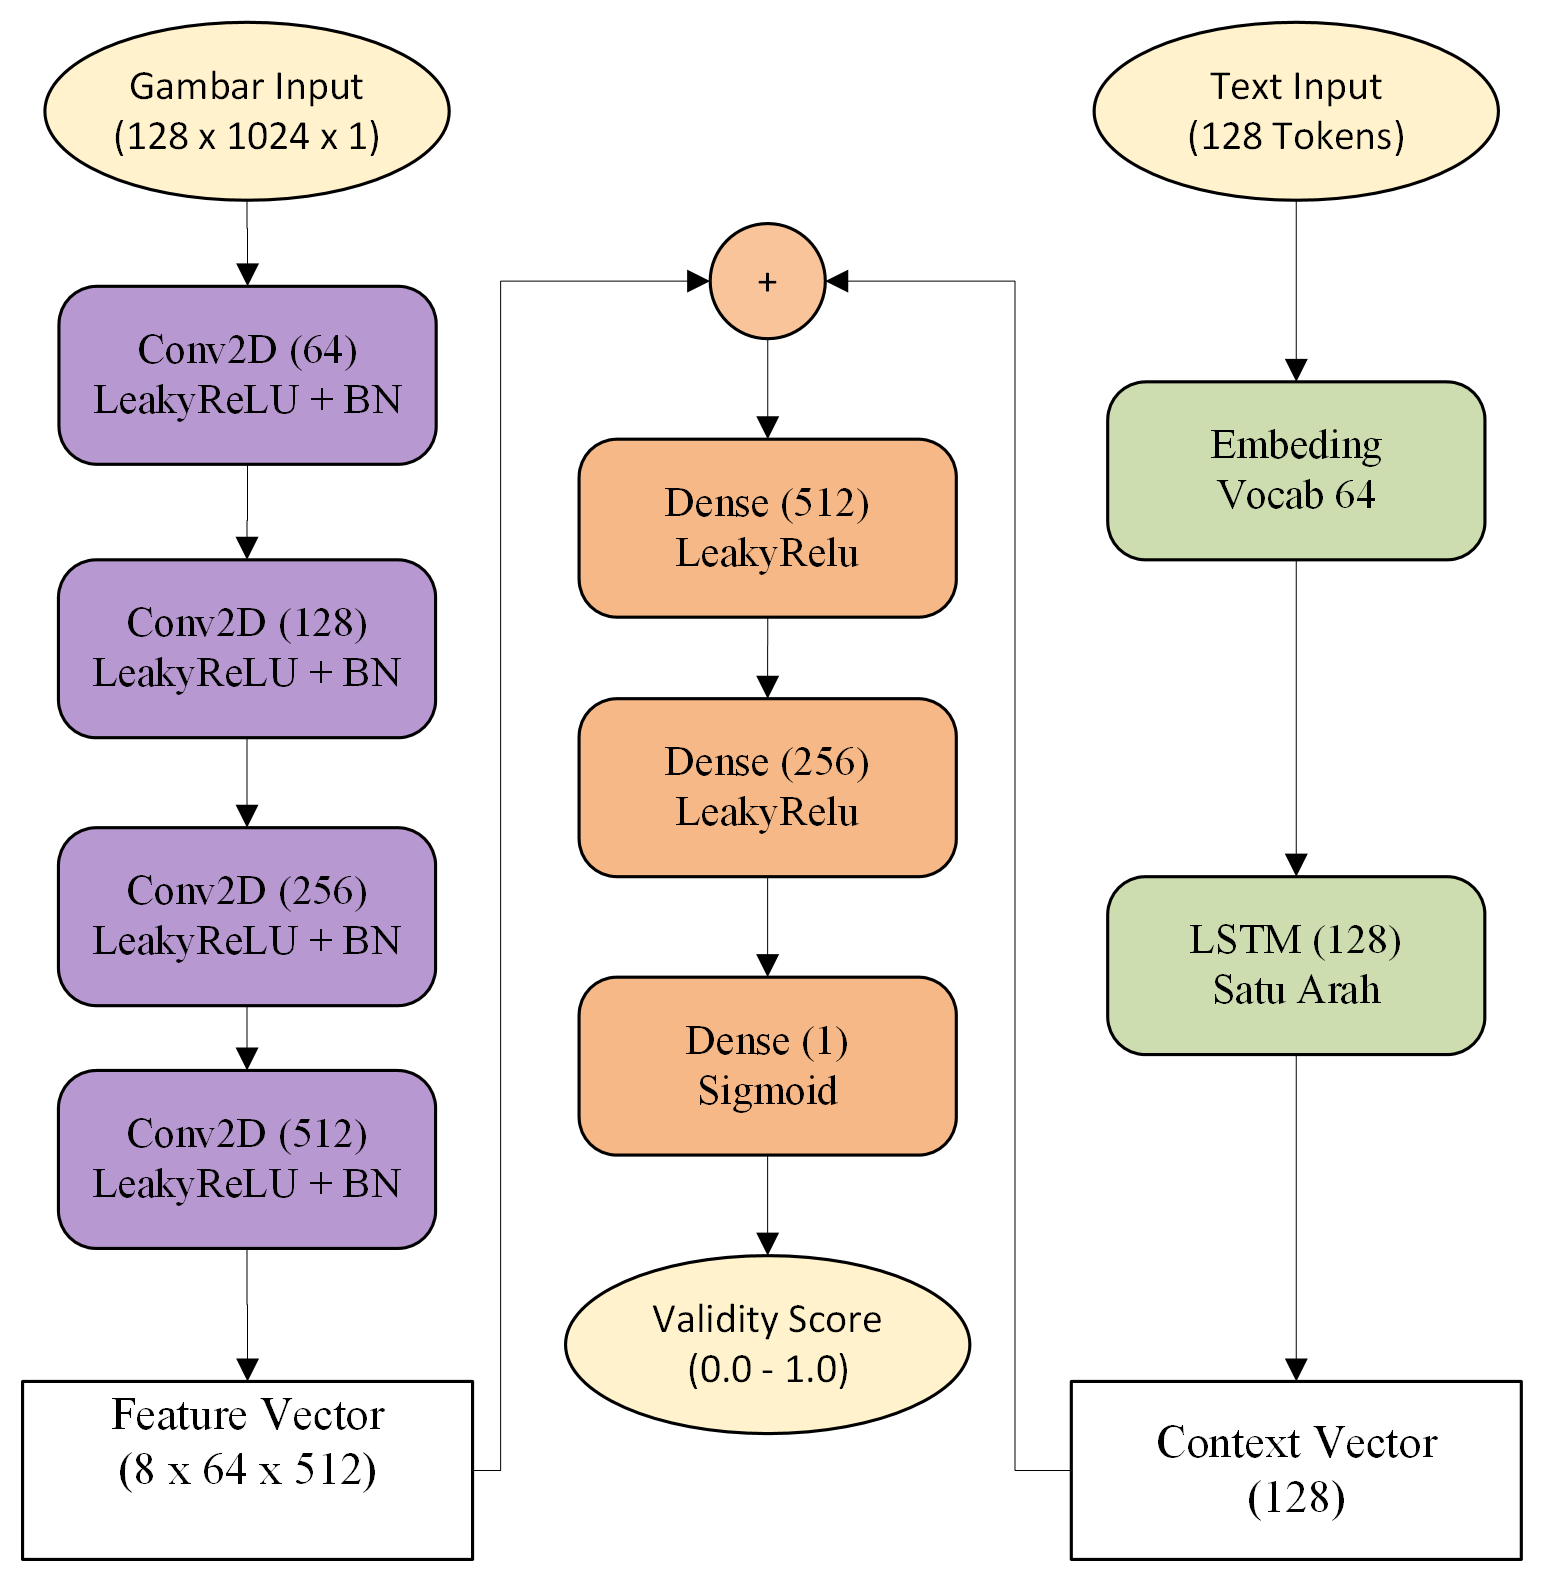
\includegraphics[width=0.9\textwidth]{images/dual-modal.png}
\caption{Diagram arsitektur Diskriminator Dual-Modal.}
\label{fig:dual-modal}
\end{figure}

\subsubsection{Desain Fungsi Loss} % This will be numbered as 4.2.5

Optimalisasi arsitektur GAN yang diusulkan mengandalkan dua fungsi loss yang bekerja secara simultan. Desain fungsi loss untuk Generator menjadi salah satu kontribusi utama karena secara eksplisit memasukkan metrik keterbacaan teks.

\paragraph{Fungsi Loss Diskriminator}
Fungsi loss untuk Diskriminator ($L_D$) menggunakan Binary Cross-Entropy (BCE) standar untuk membedakan pasangan data asli dan palsu:

\begin{equation}
L_D = -\mathbb{E}_{x,y}[\log D(x, y)] - \mathbb{E}_{z,y^{\prime}}[\log(1 - D(G(z), y^{\prime}))]
\end{equation}

\paragraph{Fungsi Loss Generator}
Fungsi loss untuk Generator ($L_G$) dirancang untuk mencapai dua tujuan: menghasilkan gambar realistis dan gambar yang teksnya dapat dibaca dengan baik. $L_G$ disusun sebagai kombinasi tiga komponen loss:

\subparagraph{1. Adversarial Loss ($L_{adv}$)}
Mengukur kemampuan Generator dalam "menipu" Diskriminator:
\begin{equation}
L_{adv} = -\mathbb{E}_{z,y^{\prime}}[\log D(G(z), y^{\prime})]
\end{equation}

\subparagraph{2. Reconstruction Loss ($L_{L1}$)}
L1 Loss untuk kemiripan piksel dengan ground truth:
\begin{equation}
L_{L1} = \mathbb{E}_{x,G(z)}[\|x - G(z)\|_1]
\end{equation}

\subparagraph{3. CTC Loss ($L_{CTC}$)}
Inovasi kunci: CTC loss dari frozen HTR model untuk mengoptimalkan keterbacaan teks:
\begin{equation}
L_{CTC} = \mathbb{E}_{z,t}[\text{CTC}(R(G(z)), t)]
\end{equation}
di mana $R(G(z))$ adalah output recognizer dari gambar hasil restorasi, dan $t$ adalah ground truth transcription.

\paragraph{Fungsi Loss Gabungan}
Ketiga komponen loss tersebut digabungkan menjadi satu fungsi loss total untuk Generator:
\begin{equation}
L_G = \lambda_{adv} L_{adv} + \lambda_{L1} L_{L1} + \lambda_{CTC} L_{CTC}
\end{equation}
Bobot $\lambda_{adv}$, $\lambda_{L1}$, dan $\lambda_{CTC}$ adalah hyperparameter yang dapat disesuaikan untuk menyeimbangkan kontribusi dari setiap komponen loss terhadap proses training Generator.

\subsection{Spesifikasi Lingkungan Implementasi}
\label{subsec:spesifikasi-lingkungan}

Untuk memastikan bahwa rancangan arsitektur GAN-HTR dapat diimplementasikan secara efektif dan reproduktif, bagian ini merinci spesifikasi teknis lingkungan implementasi. Spesifikasi ini dirancang berdasarkan analisis kebutuhan non-fungsional yang telah diidentifikasi sebelumnya, khususnya aspek reproduktifitas dan performa waktu. Dengan spesifikasi yang jelas, framework dapat dikembangkan dalam lingkungan terkontrol yang mendukung eksperimen berulang dan deployment yang konsisten.

\subsubsection{Spesifikasi Perangkat Keras}
\label{subsubsec:hardware-spec}

Spesifikasi perangkat keras yang digunakan untuk implementasi framework GAN-HTR telah didefinisikan secara lengkap pada Bab III (Metodologi Penelitian), khususnya pada Tabel 3.6 yang merinci komponen GPU (NVIDIA RTX A4000 dengan 16 GB GDDR6), CPU (Intel Xeon atau AMD Ryzen multi-core), RAM (32 GB DDR4), dan storage (1 TB NVMe SSD). Spesifikasi ini dipilih untuk memenuhi kebutuhan komputasi intensif training GAN dan memastikan reproduktifitas eksperimen.

\subsubsection{Konfigurasi Perangkat Lunak dan Library}
\label{subsubsec:software-spec}

Konfigurasi perangkat lunak dan library yang digunakan dalam implementasi juga telah diuraikan secara komprehensif pada Bab III, Tabel 3.7. Framework utama meliputi Python 3.10, TensorFlow/Keras 2.x untuk deep learning, Poetry untuk dependency management, serta library pendukung seperti NumPy, OpenCV, MLflow, dan Matplotlib. Konfigurasi ini memastikan konsistensi lingkungan development dan memfasilitasi reproduktifitas melalui file \texttt{pyproject.toml} yang terdefinisi dengan baik.

\subsubsection{Konfigurasi Docker dan Reproduktifitas}
\label{subsubsec:docker-config}

Untuk memastikan reproduktifitas, implementasi menggunakan Docker dengan konfigurasi yang mencakup base image TensorFlow 2.15.0 GPU, instalasi Poetry untuk dependency management, dan konfigurasi GPU NVIDIA dengan environment variables untuk akses penuh GPU dan compute capabilities.

\subsection{Implementasi Pipeline Data}
\label{subsec:implementasi-pipeline}

Implementasi pipeline data merupakan langkah krusial dalam mewujudkan rancangan arsitektur GAN-HTR yang telah diuraikan sebelumnya. Pipeline ini mengintegrasikan kebutuhan fungsional terkait dataset sintetis dan dukungan untuk berbagai format input, seperti yang ditentukan dalam analisis kebutuhan. Dengan pipeline yang modular, sistem dapat menangani persiapan data untuk training Recognizer dan pembuatan dataset terdegradasi sintetis, memastikan kualitas data yang konsisten untuk eksperimen yang reproduktif.

\subsubsection{Pipeline Persiapan Dataset HTR}
\label{subsubsec:dataset-htr-pipeline}

Fase pertama implementasi adalah persiapan dataset untuk training model Recognizer. Pipeline ini diimplementasikan dengan struktur modular:

\begin{algorithm}[H]
\caption{Pipeline Persiapan Dataset HTR}
\begin{algorithmic}[1]
\STATE \textbf{Input:} Halaman dokumen bersih, file XML transkripsi
\STATE \textbf{Output:} TFRecord dataset (image, transcription)
\STATE \textbf{1:} Segmentasi halaman menjadi baris teks menggunakan bounding box dari XML
\STATE \textbf{2:} Ekstrak image patch untuk setiap baris teks
\STATE \textbf{3:} Preprocessing: normalisasi intensitas, resize ke 128×1024
\STATE \textbf{4:} Binarisasi: adaptive threshold untuk contrast enhancement
\STATE \textbf{5:} Validasi: verifikasi kesesuaian image-text pairs
\STATE \textbf{6:} Konversi ke format TFRecord untuk efisiensi I/O
\STATE \textbf{7:} Split: pelatihan (80\%), validasi (10\%), pengujian (10\%)
\end{algorithmic}
\end{algorithm}

\subsubsection{Pipeline Degradasi Sintetis}
\label{subsubsec:synthetic-degradation-pipeline}

Karena keterbatasan dataset dokumen terdegradasi, dikembangkan pipeline sintetis:

\begin{algorithm}[H]
\caption{Pipeline Synthetic Degradation}
\begin{algorithmic}[1]
\STATE \textbf{Input:} Dataset HTR bersih
\STATE \textbf{Output:} Dataset triplet (degraded, clean, transcription)
\STATE \textbf{1:} Load clean images dan transcriptions
\STATE \textbf{2:} Apply degradations dengan probabilitas random:
    \STATE \quad a. Bleed-through (30\%): overlay mirrored text dengan opacity variabel
    \STATE \quad b. Fading (40\%): reduce intensity dengan exponential decay
    \STATE \quad c. Stains (25\%): add random brown spots dengan varying intensity
    \STATE \quad d. Blur (20\%): Gaussian filter dengan $\sigma \in [0.5, 2.0]$
\STATE \textbf{3:} Add noise: salt \& pepper (10\% pixels) untuk simulasi sensor noise
\STATE \textbf{4:} Validasi quality metrics (PSNR > 20 dB) untuk memastikan degradasi tidak ekstrem
\STATE \textbf{5:} Simpan sebagai TFRecord triplet dengan struktur (degraded, clean, transcription)
\end{algorithmic}
\end{algorithm}

\subsubsection{Format Data dan Preprocessing}
\label{subsubsec:format-preprocessing}

\paragraph{Format TFRecord:}
Setiap sample disimpan dalam TFRecord dengan struktur:
\begin{itemize}
    \item \texttt{degraded\_image}: Tensor uint8 [128, 1024, 1]
    \item \texttt{clean\_image}: Tensor uint8 [128, 1024, 1]
    \item \texttt{transcription}: String teks ground truth
    \item \texttt{length}: Int panjang sequence
\end{itemize}

\subsection{Detail Implementasi Training}
\label{subsec:detail-implementasi-training}

Bagian ini menguraikan detail implementasi proses training yang mengoperasionalkan rancangan arsitektur GAN adversarial dengan dual-modal discriminator. Implementasi ini mempertimbangkan kebutuhan non-fungsional seperti performa waktu dan reproduktifitas, dengan konfigurasi yang disesuaikan untuk mencapai target PSNR, SSIM, dan penurunan CER/WER. Teknik seperti multi-component loss dan precision policy diintegrasikan untuk memastikan stabilitas training dan optimasi keterbacaan teks.

\subsubsection{Konfigurasi Pelatihan Generator}
\label{subsubsec:generator-training}

\begin{table}[H]
\centering
\caption{Konfigurasi training Generator}
\label{tab:generator-config}
\small
\begin{tabular}{|l|l|}
\hline
\textbf{Parameter} & \textbf{Nilai} \\
\hline
Optimizer & Adam \\
\hline
Learning Rate & $1 \times 10^{-4}$ \\
\hline
Batch Size & 16 \\
\hline
Loss Weights & $\lambda_{adv}=1.0$, $\lambda_{L1}=100.0$, $\lambda_{CTC}=1.0$ \\
\hline
Gradient Clipping & clipnorm=1.0 \\
\hline
Epochs & 100 (dengan early stopping) \\
\hline
\end{tabular}
\end{table}

\subsubsection{Implementasi Multi-Component Loss Function}
\label{subsubsec:loss-implementation}

Fungsi loss multi-komponen diimplementasikan untuk mengoptimalkan Generator secara simultan pada tiga aspek utama: adversarial loss untuk menipu diskriminator, L1 reconstruction loss untuk kesamaan piksel dengan ground truth, dan CTC readability loss untuk meningkatkan keterbacaan teks. Pendekatan ini memastikan keseimbangan antara kualitas visual dan tekstual melalui bobot yang dapat dikonfigurasi, dengan clipping pada CTC loss untuk stabilitas numerik.

\begin{figure}[H]
\centering
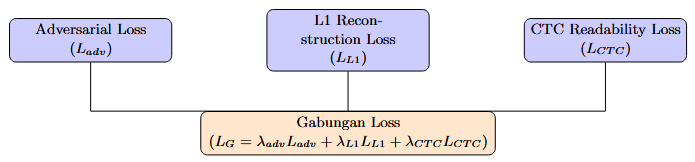
\includegraphics[width=0.9\textwidth]{images/gambarMultiComponentLoss.png}
\caption{Diagram komponen multi-component loss untuk Generator.}
\label{fig:multi-loss}
\end{figure}

\subsubsection{Discriminator Mode Implementation}
\label{subsubsec:discriminator-mode-impl}

Dual-modal discriminator mendukung dua mode operasi yang dapat dikonfigurasi sesuai dengan desain eksperimen yang telah diuraikan pada Bab III.4.3:

\paragraph{Ground Truth Mode:}
Mode ini menggunakan ground truth text sebagai input teks untuk diskriminator. Karakteristik:
\begin{itemize}[leftmargin=*, nosep]
\item \textbf{Stabilitas:} Training lebih stabil karena teks konsisten dan bebas error
\item \textbf{Kelebihan:} Konvergensi cepat, loss smooth, cocok untuk initial training
\item \textbf{Kekurangan:} Kurang realistis untuk deployment karena tidak mensimulasikan kondisi inference
\item \textbf{Use Case:} Ideal untuk warmup phase dan debugging architecture
\end{itemize}

\paragraph{Predicted Mode:}
Mode ini menggunakan predicted text dari frozen recognizer sebagai input. Karakteristik:
\begin{itemize}[leftmargin=*, nosep]
\item \textbf{Realisme:} Mensimulasikan kondisi deployment dengan error recognition
\item \textbf{Kelebihan:} Model belajar handle imperfect text, generalisasi lebih baik
\item \textbf{Kekurangan:} Training lebih challenging, memerlukan recognizer berkualitas tinggi (CER < 15\%)
\item \textbf{Use Case:} Ideal untuk fine-tuning dan evaluation yang realistis
\end{itemize}

\paragraph{Eksperimen Perbandingan:}
Perbandingan kuantitatif kedua mode akan dilakukan melalui eksperimen terkontrol dengan metrik CER, WER, PSNR, dan SSIM. Hasil lengkap dan analisis statistical significance akan dibahas pada Bab V (Hasil dan Pembahasan), sesuai dengan desain eksperimen yang dirancang pada Bab V.



\subsubsection{Implementasi Kebijakan Presisi}
\label{subsubsec:precision-policy-implementation}

Kebijakan presisi pure FP32 diimplementasikan secara eksplisit untuk memastikan stabilitas numerik dalam training, terutama untuk kalkulasi CTC loss yang memerlukan presisi penuh. Pendekatan ini menghindari underflow/overflow pada gradient calculations, memastikan konsistensi multi-component loss, dan mendukung stabilitas keseluruhan proses adversarial.

\textbf{Catatan:} Pipeline pelatihan Recognizer (metodologi, rationale, curriculum learning strategy) telah diuraikan pada Bab III Fase 2. Bagian ini fokus pada detail implementasi teknis.

\subsection{Implementasi Pelatihan dan Evaluasi}
\label{subsec:implementasi-training}

Implementasi pelatihan dan evaluasi melengkapi siklus pengembangan framework GAN-HTR, dengan fokus pada konfigurasi training diskriminator dan sistem evaluasi multi-metrik. Bagian ini menjembatani rancangan arsitektur dengan praktik implementasi, memastikan bahwa metrik evaluasi seperti CER dan WER dapat diukur secara konsisten sesuai target non-fungsional. Penggunaan MLflow untuk tracking eksperimen mendukung reproduktifitas dan analisis performa yang mendalam.

\subsubsection{Konfigurasi Pelatihan Diskriminator}
\label{subsubsec:discriminator-training}

Konfigurasi training diskriminator dirancang untuk mencapai Nash equilibrium dalam adversarial training, sesuai dengan strategi yang telah dijelaskan pada Bab III.4.3. Target accuracy 60-80\% menunjukkan keseimbangan optimal antara generator dan discriminator.

\begin{table}[H]
\centering
\caption{Konfigurasi training Diskriminator}
\label{tab:discriminator-config}
\small
\begin{tabular}{|l|l|}
\hline
\textbf{Parameter} & \textbf{Nilai} \\
\hline
Optimizer & Adam \\
\hline
Learning Rate & $5 \times 10^{-4}$ (2.5x learning rate Generator) \\
\hline
Batch Size & 16 (sama dengan Generator) \\
\hline
Loss & Binary Cross-Entropy dengan label smoothing (0.9) \\
\hline
Target Accuracy & 60-80\% (Nash equilibrium zone) \\
\hline
Gradient Penalty & Tidak digunakan (diganti label smoothing) \\
\hline
\end{tabular}
\end{table}

Rasio learning rate 2.5:1 (Discriminator:Generator) dipilih untuk mempercepat konvergensi discriminator tanpa menyebabkan mode collapse, berdasarkan best practice GAN training.

\subsubsection{Implementasi MLflow Tracking}
\label{subsubsec:mlflow-implementation}

MLflow diintegrasikan untuk pelacakan eksperimen secara sistematis, memungkinkan dokumentasi parameter, metrik, dan artefak model dalam lingkungan terstruktur. Pendekatan ini memfasilitasi reproduktifitas eksperimen melalui pencatatan hyperparameter, evolusi metrik per epoch, dan penyimpanan model, sehingga mendukung analisis komparatif dan optimasi berbasis data historis.

\subsubsection{Sistem Evaluasi Multi-Metrik}
\label{subsubsec:evaluasi-multi-metrik}

Sistem evaluasi mengimplementasikan metrik yang dijelaskan pada Bab III.5, dengan fokus pada pengukuran kualitas visual dan tekstual secara simultan. Metrik PSNR dan SSIM digunakan untuk menilai kesamaan visual dengan target di atas 35 dB dan 0.90, sementara CER dan WER mengukur keterbacaan teks dengan target di bawah 5\% dan 15\%. Pendekatan multi-metrik ini memastikan evaluasi komprehensif yang seimbang antara aspek visual dan tekstual dalam konteks restorasi dokumen.



\subsection{Sistem Monitoring dan Tracking}
\label{subsec:monitoring-tracking}

Sistem monitoring dan tracking diimplementasikan untuk mendukung evaluasi kontinyu selama proses training, sesuai dengan kebutuhan non-fungsional reproduktifitas. Dengan real-time monitoring loss components dan metrics evolution, sistem ini memungkinkan deteksi dini masalah seperti mode collapse atau imbalance, memastikan bahwa training GAN adversarial berjalan stabil dan efisien. Checkpoint management dan early stopping diintegrasikan untuk optimasi sumber daya komputasi.

\subsubsection{Real-time Training Monitoring}
\label{subsubsec:realtime-monitoring}

Sistem monitoring real-time diimplementasikan untuk tracking progress training, dengan fokus pada komponen loss generator (adversarial, L1, CTC, total), loss diskriminator (klasifikasi real/fake), dan rasio loss untuk deteksi imbalance. Evolusi metrik seperti PSNR/SSIM per epoch, tren peningkatan CER/WER, serta indikator stabilitas training memungkinkan pengawasan kontinyu dan intervensi dini terhadap masalah seperti mode collapse atau ketidakseimbangan dalam proses adversarial.

\subsubsection{Checkpoint Management Strategy}
\label{subsubsec:checkpoint-management}

Strategi manajemen checkpoint dirancang untuk efisiensi penyimpanan, dengan fokus pada penyimpanan model terbaik saja berdasarkan validation loss, pemantauan otomatis, dan pembersihan checkpoint lama. Pendekatan ini mengoptimalkan penggunaan sumber daya komputasi sambil memastikan ketersediaan model optimal untuk evaluasi dan deployment.

\subsubsection{Implementasi Early Stopping }
\label{subsubsec:early-stopping}

Pemberhentian dini (early stopping) diimplementasikan untuk mencegah overfitting dan menghemat sumber daya, dengan kriteria patience 15 epoch tanpa improvement pada validation total generator loss, serta pemulihan otomatis bobot terbaik. Strategi ini memastikan efisiensi training sambil mempertahankan performa model yang optimal.

\subsection{Optimasi dan Fine-Tuning}
\label{subsec:optimasi-finetuning}

Optimasi dan fine-tuning merupakan tahap akhir dalam desain implementasi, yang bertujuan untuk meningkatkan performa framework GAN-HTR melampaui baseline awal. Strategi ini mengintegrasikan teknik regularisasi, hyperparameter tuning, dan debugging untuk mencapai target kualitas visual dan tekstual yang ditetapkan dalam analisis kebutuhan. Dengan pendekatan ini, sistem dapat dioptimalkan untuk skala produksi sambil mempertahankan stabilitas training.

\subsubsection{Strategi Optimasi Hyperparameter}
\label{subsubsec:hyperparameter-optimasi}

Strategi optimasi hyperparameter mencakup penjadwalan learning rate dengan ReduceLROnPlateau dan patience 5, tuning bobot loss melalui grid search untuk nilai lambda, optimasi batch size dengan eksperimen pada ukuran 8, 16, dan 32, serta pencarian arsitektur dengan variasi jumlah filter dan lapisan. Pendekatan ini memfasilitasi pencapaian performa optimal melalui eksplorasi sistematis parameter kunci.

\subsubsection{Teknik Regularisasi dan Stabilisasi}
\label{subsubsec:regularisasi-stabilisasi}

Teknik regularisasi dan stabilisasi mencakup gradient penalties untuk stabilitas training GAN, spectral normalization pada diskriminator, label smoothing untuk menghindari overconfidence, serta experience replay dengan buffer dari sampel yang dihasilkan. Pendekatan ini memastikan konvergensi yang stabil dan performa yang konsisten dalam proses adversarial.

\subsubsection{Monitoring dan Debugging}
\label{subsubsec:monitoring-debugging}

Sistem monitoring mencakup tracking loss real-time dengan TensorBoard, visualisasi sampel per epoch, pemantauan aliran gradien, dan deteksi mode collapse. Strategi debugging meliputi smoke test dengan dataset kecil, pengujian komponen terpisah, ablation loss untuk setiap komponen, serta pencarian learning rate optimal. Pendekatan ini memfasilitasi identifikasi dan resolusi masalah secara sistematis selama fase optimasi.

\subsection{Framework Modular dan Reusable}
\label{subsec:framework-modular}

Framework modular dan reusable dirancang untuk memfasilitasi ekstensi dan penggunaan ulang komponen, sesuai dengan prinsip desain yang efisien dalam konteks analisis dan implementasi. Dengan arsitektur yang loosely coupled, sistem ini dapat diadaptasi untuk berbagai skenario restorasi dokumen, mendukung plugin architecture dan testing framework yang komprehensif. Deployment framework memastikan transisi mulus dari eksperimen ke penggunaan produksi.

\subsubsection{Arsitektur Modular}
\label{subsubsec:arsitektur-modular}

Framework GAN-HTR dirancang dengan arsitektur modular untuk memastikan reusability dan extensibility, di mana setiap komponen seperti generator (U-Net), diskriminator (dual-modal), recognizer (frozen HTR), loss (multi-component), data pipeline, dan training loop beroperasi sebagai modul independen dengan interface terdefinisi. Prinsip desain mencakup loose coupling untuk dependensi minimal, high cohesion untuk pengelompokan fungsi terkait, abstraction layers untuk implementasi berbeda, serta dependency injection untuk konfigurasi runtime. Pendekatan ini memfasilitasi adaptasi framework terhadap berbagai skenario restorasi dokumen.

\subsubsection{Konfigurasi Sistem}
\label{subsubsec:sistem-konfigurasi}

Konfigurasi sistem dirancang untuk mengelola parameter model dan eksperimen secara efisien, mendukung kebutuhan reproduktifitas (NFR-4) melalui mekanisme inheritance dan override. Dengan pendekatan ini, konfigurasi dapat disesuaikan untuk berbagai eksperimen tanpa mengubah kode inti, memastikan konsistensi dalam analisis dan desain framework.

Sistem konfigurasi mengadopsi pendekatan hierarkis yang memungkinkan pewarisan parameter dari konfigurasi dasar ke konfigurasi spesifik eksperimen. Mekanisme override memfasilitasi penyesuaian parameter tertentu sesuai kebutuhan eksperimen, sambil mempertahankan struktur dasar yang konsisten. Pendekatan ini mengoptimalkan efisiensi pengelolaan konfigurasi, mengurangi redundansi, dan memastikan bahwa setiap eksperimen dapat direproduksi dengan parameter yang terdokumentasi secara jelas.

% \paragraph{Parameter Management:}
\paragraph{ }
\begin{table}[H]
\centering
\caption{Kategori parameter konfigurasi}
\label{tab:config-categories}
\small
\begin{tabular}{|l|l|}
\hline
\textbf{Kategori} & \textbf{Parameter} \\
\hline
Model Architecture & Filters, layers, activation functions \\
\hline
Training Hyperparameters & Learning rate, batch size, epochs \\
\hline
Loss Configuration & Loss weights, clipping values \\
\hline
Data Pipeline & Augmentation, preprocessing, loading \\
\hline
Experiment Tracking & MLflow settings, logging frequency \\
\hline
\end{tabular}
\end{table}

\subsubsection{Arsitektur Plugin}
\label{subsubsec:plugin-architecture}

Arsitektur plugin dikembangkan untuk meningkatkan ekstensi framework tanpa modifikasi inti, sesuai dengan prinsip modularitas yang dirancang untuk mendukung kebutuhan integrasi sistem. Dengan mekanisme registrasi komponen kustom, sistem dapat diperluas untuk berbagai skenario restorasi dokumen, memastikan fleksibilitas dan kemudahan maintenance dalam konteks analisis desain.

Arsitektur ini menyediakan dukungan untuk komponen kustom melalui mekanisme registrasi yang terstruktur, memungkinkan pengembang untuk menambahkan lapisan baru, fungsi loss, metrik evaluasi, dan sumber data tanpa mengganggu arsitektur inti. Pendekatan ini memfasilitasi ekstensi framework secara dinamis, di mana komponen kustom dapat didaftarkan dan diintegrasikan pada saat runtime, sehingga meningkatkan adaptabilitas sistem terhadap kebutuhan spesifik aplikasi restorasi dokumen.

\subsubsection{Testing Framework}
\label{subsubsec:testing-framework}

Framework menyediakan comprehensive testing suite untuk memastikan kualitas dan reusability.

Strategi pengujian unit mencakup validasi berbagai aspek komponen, mulai dari bentuk output model, jumlah parameter, hingga aliran gradien, untuk memastikan integritas setiap modul. Pengujian data memverifikasi proses pemuatan, preprocessing, dan augmentasi, sementara pengujian training mengevaluasi komputasi loss dan pembaruan optimizer. Pengujian integrasi memvalidasi pipeline end-to-end secara keseluruhan, memastikan bahwa semua komponen berinteraksi dengan benar dalam konteks desain framework.

Pipeline pengujian terotomatisasi mengintegrasikan berbagai jenis pengujian dalam urutan yang sistematis, dimulai dari pengujian unit untuk komponen individual, dilanjutkan dengan pengujian integrasi untuk interaksi antar-komponen, dan diakhiri dengan pengujian performa serta validasi untuk memastikan kesesuaian dengan spesifikasi desain. Pendekatan ini memfasilitasi deteksi dini masalah dan pembuatan laporan komprehensif untuk mendukung kualitas framework secara keseluruhan.

\subsubsection{Deployment Framework}
\label{subsubsec:deployment-framework}

Deployment Framework  dirancang untuk memenuhi kebutuhan integrasi sistem (FR-8) yang telah diidentifikasi dalam analisis kebutuhan, memungkinkan framework GAN-HTR untuk dioperasikan dalam lingkungan produksi. Dengan pendekatan ini, sistem dapat diekspor dalam berbagai format untuk mendukung deployment skala besar, sambil mempertahankan performa dan reproduktifitas yang telah dirancang.

Framework deployment ini mengintegrasikan komponen-komponen utama melalui mekanisme ekspor model yang fleksibel, yang memungkinkan adaptasi terhadap berbagai platform komputasi. Pendekatan ini memfasilitasi transisi dari lingkungan pengembangan ke produksi dengan meminimalkan overhead integrasi, sekaligus menjaga konsistensi performa yang telah dioptimalkan selama fase pelatihan. Selain itu, antarmuka aplikasi yang terstruktur menyediakan kanal komunikasi standar untuk interaksi dengan sistem eksternal, memungkinkan integrasi seamless dalam alur kerja operasional yang lebih luas.

% \subsection{Kesimpulan Desain dan Implementasi}
% \label{subsec:kesimpulan-desain}

% Bab ini telah menguraikan analisis dan desain komprehensif untuk framework GAN-HTR yang mampu melakukan restorasi dokumen terdegradasi dengan orientasi pada keterbacaan teks. Rancangan solusi ini memenuhi semua kebutuhan fungsional dan non-fungsional yang telah diidentifikasi, dengan memberikan perhatian khusus pada keseimbangan antara kualitas visual dan keterbacaan tekstual.

% \paragraph{Kontribusi Utama Desain:}
% \begin{enumerate}
%     \item \textbf{Inovasi Arsitektural:} Dual Modal Discriminator yang mengevaluasi koherensi visual-teksual
%     \item \textbf{Integrasi HTR-GAN:} CTC loss dari frozen HTR model
%     \item \textbf{Optimasi Ganda:} Fungsi loss multi-komponen yang seimbang
%     \item \textbf{Reproduktifitas:} Lingkungan terkontrol dengan Docker dan MLflow
% \end{enumerate}

% \paragraph{Implementasi Teknis:}
% Detail implementasi yang telah diuraikan meliputi spesifikasi lingkungan, pipeline data, konfigurasi training, dan strategi optimasi. Semua komponen dirancang untuk memastikan reproduktifitas dan kemudahan deployment.

% Rancangan ini memberikan fondasi yang kuat untuk implementasi framework GAN-HTR yang dapat mengatasi tantangan restorasi dokumen historis dengan berorientasi pada peningkatan keterbacaan teks, bukan hanya perbaikan visual semata.

\end{document}
